%  LaTeX support: latex@mdpi.com
%  For support, please attach all files needed for compiling as well as the log file, and specify your operating system, LaTeX version, and LaTeX editor.

%=================================================================
\documentclass[hydrology,article,submit,pdftex,moreauthors]{Definitions/mdpi}

% Additional packages
\usepackage{listings}
\usepackage{longtable}

% Code listing style
\lstset{
  basicstyle=\ttfamily\small,
  breaklines=true,
  frame=single,
  language=Python
}

%=================================================================
% MDPI internal commands - do not modify
\firstpage{1}
\makeatletter
\setcounter{page}{\@firstpage}
\makeatother
\pubvolume{1}
\issuenum{1}
\articlenumber{0}
\pubyear{2026}
\copyrightyear{2026}
%\externaleditor{Academic Editor: Firstname Lastname}
\datereceived{ }
\daterevised{ }
\dateaccepted{ }
\datepublished{ }
\hreflink{https://doi.org/}

%=================================================================
% Full title of the paper (Capitalized)
\Title{BASEFLOW: A Python Package for Digital Baseflow Separation and Analysis}

% MDPI internal command: Title for citation in the left column
\TitleCitation{BASEFLOW: A Python Package for Digital Baseflow Separation and Analysis}

% Author ORCID IDs
\newcommand{\orcidauthorA}{0000-0002-7597-2825} % Norman Jones

% Authors, for the paper (add full first names)
\Author{Xueyi Li~$^{1}$, Amin Aghababaei~$^{1}$, Ryan van der Heijden~$^{2}$, Eniola Webster-Esho~$^{3}$, Joshua Hart~$^{1}$, Amber Kunz~$^{1}$, Berkeley Berrett~$^{1}$, Norman Jones~$^{1,}$*\orcidA{}, Gus Williams~$^{1}$, Donna Rizzo~$^{2}$, and T.~Prabhakar Clement~$^{3}$}

% MDPI internal command: Authors, for metadata in PDF
\AuthorNames{Xueyi Li, Amin Aghababaei, Ryan van der Heijden, Eniola Webster-Esho, Joshua Hart, Amber Kunz, Berkeley Berrett, Norman Jones, Gus Williams, Donna Rizzo and T. Prabhakar Clement}

% MDPI internal command: Authors, for citation in the left column
\AuthorCitation{Li, X.; Aghababaei, A.; van der Heijden, R.; Webster-Esho, E.; Hart, J.; Kunz, A.; Berrett, B.; Jones, N.; Williams, G.; Rizzo, D.; Clement, T.P.}

% Affiliations / Addresses
\address{%
$^{1}$ \quad Civil and Construction Engineering, Brigham Young University, Provo, UT 84602, USA\\
$^{2}$ \quad Civil and Environmental Engineering, University of Vermont, Burlington, VT 05405, USA\\
$^{3}$ \quad Civil, Construction and Environmental Engineering, University of Alabama, Tuscaloosa, AL 35487, USA}

% Contact information of the corresponding author
\corres{Correspondence: njones@byu.edu; Tel.: +1-801-225-0799 (N.J.)}

%\simplesumm{}

%\conference{}

% Abstract (Do not insert blank lines, i.e. \\)
\abstract{Baseflow is a critical component of groundwater discharge, but it is difficult to measure directly. Therefore, it is common practice to estimate baseflow from total streamflow using various methods, such as graphical and digital techniques. We have developed the baseflow Python package, which implements multiple baseflow separation methods and includes utility functions for data preprocessing, making it easier for users to apply these techniques. Comprehensive documentation is provided, along with detailed examples. Additionally, we offer Google Colab notebooks that demonstrate step-by-step usage and allow users to run their own data interactively.}

% Keywords
\keyword{python; baseflow; quickflow; separation}

%%%%%%%%%%%%%%%%%%%%%%%%%%%%%%%%%%%%%%%%%%
\begin{document}

%%%%%%%%%%%%%%%%%%%%%%%%%%%%%%%%%%%%%%%%%%
\section{Introduction}
\label{sec:introduction}

Streamflow is a combination of direct runoff from precipitation, snowmelt, and the delayed contribution from groundwater and bank flow. Baseflow refers specifically to the portion of streamflow that originates from groundwater and other delayed sources, while the remaining part, which responds more quickly to precipitation, is termed quickflow. Baseflow plays a crucial role in sustaining river ecosystems and managing water resources. It represents the long-term discharge that persists between precipitation events, making it fundamental to understanding watershed hydrology, managing water quality, and supporting ecological processes in rivers and streams.

However, directly measuring baseflow is challenging~\cite{ref1}, so various methods are employed to estimate it by separating baseflow from total streamflow. These methods can generally be grouped into three categories: hydrochemical, graphical, and digital. Hydrochemical methods rely on measurements such as electrical conductivity to estimate local baseflow contributions~\cite{ref2}. Graphical methods visually separate baseflow from the hydrograph, based on the assumption that groundwater flow changes more slowly than surface runoff. Common graphical techniques include fixed interval, sliding interval, and local minimum methods. Digital methods, on the other hand, employ mathematical functions and signal processing algorithms to compute baseflow from total streamflow data. The first widely adopted digital method, the Lyne--Hollick filter~\cite{ref3}, produced results similar to those of the local minimum method, and subsequent methods such as the Chapman~\cite{ref4} and Eckhardt~\cite{ref5} methods have further simplified the estimation process, requiring only streamflow data.

Several studies have demonstrated the application of these methods in real-world contexts. For example, Shao et al.\ applied the Hydrograph Separation Program (HYSEP)~\cite{ref6}, the UK Institute of Hydrology's method (UKIH)~\cite{ref7}, and the Eckhardt digital method to the Hailiutu River in Northwestern China, using trace-based hydrochemistry as a reference and finding that the Eckhardt method performed best~\cite{ref8}. Similarly, Ichwana Ramli used the Chapman method to evaluate groundwater contributions in the Peusangan Watershed during peak streamflow events~\cite{ref9}. Dawit Midagsa Abdi applied multiple methods in the Rift Valley Lakes Basin of Ethiopia and concluded that the exponentially weighted moving average (EWMA) and Lyne--Hollick methods were the most effective~\cite{ref10}.

Regardless of the method chosen, applying these techniques often requires significant coding and computational effort, especially when multiple methods are employed. Most studies continue to rely on classic approaches, using well-established equations. To streamline this process, we developed a free Python package called baseflow, which provides separation functions for all the popular graphical and digital methods. The package is designed to be user-friendly, requiring only streamflow data as input and offering detailed explanations of parameters as well as theoretical background for each method. Additionally, it includes preprocessing tools such as data cleaning. Our goal is to make the process of baseflow separation more accessible and straightforward for researchers and practitioners alike.

%%%%%%%%%%%%%%%%%%%%%%%%%%%%%%%%%%%%%%%%%%
\section{Baseflow Python Package}
\label{sec:package}

\subsection{Package Description}
\label{sec:package_description}

The Baseflow Python package is a comprehensive toolkit designed for baseflow separation and analysis. It provides researchers and hydrologists with a suite of functions to perform various baseflow separation techniques on streamflow data.

The package is open source and can be easily installed using standard Python package management tools. Users can import the package and access its modules and functions after installation.

The Baseflow package is accompanied by comprehensive documentation hosted on the ReadtheDocs website, providing users with an extensive reference for its usage. This documentation offers a concise overview of the package, encompassing not only the theoretical background and relevant citations but also detailed function definitions and explanations of each parameter.

We also created a Google Colab notebook to serve as an interactive and user-friendly tutorial with the example streamflow data downloaded from a USGS station. It provides step-by-step guidance through the entire workflow, from obtaining data from USGS sources to calculating separation results and visualizing the outcomes. The tutorial allows individuals to execute each cell sequentially and observe the results in real-time. This interactive approach enables users to easily check outcomes and compare the performance of different separation methods.

By providing this combination of detailed documentation and hands-on tutorials, users can quickly familiarize themselves with the Baseflow package and effectively apply it to their hydrological analyses.

\subsection{Baseflow Separation Functions}
\label{sec:separation_functions}

As mentioned earlier, numerous researchers have developed various methods for baseflow separation, resulting in a wide range of equations. However, the complexity of these functions can make their implementation time-consuming and challenging. To address this, we have dedicated a section in our package specifically for baseflow separation, incorporating all the commonly available methods in Python. These methods are summarized in Table~\ref{tab:separation} below.

\begin{table}[H]
\caption{All the functions under the `separation' type.\label{tab:separation}}
\small
\begin{tabularx}{\textwidth}{llXl}
\toprule
\textbf{Function Name} & \textbf{Method} & \textbf{Parameters} & \textbf{Reference} \\
\midrule
boughton        & Boughton                                      & Q, a, c                                              & \cite{ref11} \\
chapman         & Chapman                                       & Q, a                                                 & \cite{ref4}  \\
chapman\_maxwell & Chapman \& Maxwell                            & Q, a                                                 & \cite{ref1}  \\
eckhardt        & Eckhardt                                      & A, a, BFImax                                         & \cite{ref5}  \\
ewma            & Exponential weighted moving average (EWMA)    & Q, e                                                 & \cite{ref12} \\
fixed           & Fixed interval graphical method (HYSEP)       & Q, area                                              & \cite{ref13} \\
furey           & Furey                                         & Q, a, A                                              & \cite{ref14} \\
lh              & Lyne--Hollick (LH)                            & Q, beta                                              & \cite{ref15} \\
lh\_multi       & Multi-pass Lyne--Hollick                      & Q, beta, num\_pass                                   & \cite{ref16} \\
local           & Local minimum graphical method (HYSEP)        & Q, area                                              & \cite{ref17} \\
slide           & Slide interval graphical method (HYSEP)       & Q, area                                              & \cite{ref18} \\
ukih            & UK Institute of Hydrology (UKIH) method       & Q                                                    & \cite{ref7}  \\
what            & Web-based Hydrograph Analysis Tool (WHAT)     & Q, BFImax, alpha                                     & \cite{ref19} \\
willems         & Willems                                       & Q, a, w                                              & \cite{ref19} \\
bn77            & BN77                                          & Q, L\_min, snow\_freeze\_period, observational\_precision, quantile & \cite{ref20} \\
strict\_baseflow & Strict baseflow                              & Q, ice, quantile                                     & \cite{ref21} \\
Hyd\_run        & HydRun                                        & Q, k, passes                                         & \cite{ref22} \\
\bottomrule
\end{tabularx}
\end{table}

Each function implements a specific baseflow separation algorithm, providing users with a diverse toolkit to analyze streamflow data according to their research needs and preferences. The package includes both classic methods like the Lyne--Hollick filter and more recent developments like the Eckhardt filter, ensuring a comprehensive coverage of baseflow separation techniques.

Most functions follow a similar parameter structure, typically requiring the streamflow time series (Q) and method-specific parameters. Many also include options for specifying the initial baseflow value and whether to return additional information about the separation process.

It is important to note that several common parameters are used across these separation functions. One of the inputs for each function is streamflow data (\texttt{Q}), which is structured as a NumPy array. Another commonly used input, particularly in digital filters, is the recession coefficient (\texttt{a}), which indicates the rate at which baseflow decreases between storm events. This coefficient can be calculated using functions from the \texttt{Estimate} module or, optionally, defined as a constant value by the user when calling the function.

Many methods, such as Eckhardt, EWMA, and Chapman, require an initial baseflow value (\texttt{Q0}) for iterative calculations. We provide several options for this parameter. Typically, the minimum value of the streamflow series (min) is used, but other popular choices include the initial result from the Lyne--Hollick method (LH) or the first streamflow value (Q0). Users also have the flexibility to specify any constant value as the initial baseflow.

The return values of these functions are straightforward. They include the baseflow values in a NumPy array. Additionally, if the \texttt{return\_exceed} option is set to \texttt{True}, the function will also return the number of times the calculated baseflow values exceed the corresponding original streamflow. Due to the nature of the algorithm, the calculated baseflow values may occasionally exceed the streamflow values, which is not physically realistic. We have addressed this issue in the code, and the function can report how many times this adjustment was necessary.

Taking the Chapman function as an example, this function accepts four inputs: the streamflow time series (\texttt{Q}) as a NumPy array, the recession coefficient (\texttt{a}) as a float, an optional initial baseflow value (\texttt{initial\_method}), and an option to return the number of times the baseflow exceeds the streamflow (\texttt{return\_exceed}). When executed, the function returns the baseflow values (\texttt{b}) according to the Chapman method in a NumPy array, along with the optional return of the exceedance count as an integer. Figure~\ref{fig:chapman_code} presents example code for the Chapman method, which is also included in the documentation.

\begin{figure}[H]
\centering
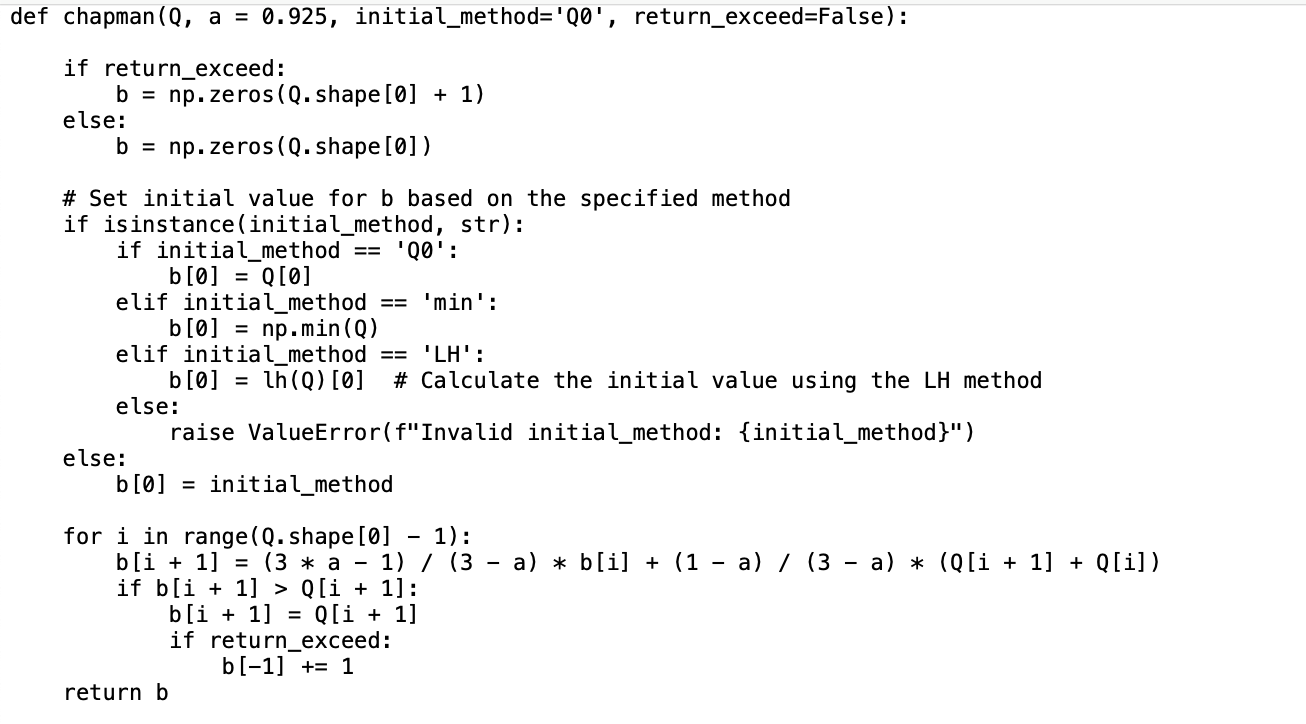
\includegraphics[width=0.8\textwidth]{figures/fig1.png}
\caption{Chapman method code.\label{fig:chapman_code}}
\end{figure}

The first step in utilizing this function is to ensure that the input streamflow data is formatted as a NumPy array. It is advisable to clean the data before performing calculations to maintain data quality. After the data preparation, the Chapman separation can be performed with a single line of code. In this example, the sample data included in the package is utilized. A constant value of 0.98 is set for the recession coefficient (\texttt{a}), and the first streamflow value is selected as the initial baseflow (\texttt{Q0}), with the default setting excluding the return of the exceedance count.

\begin{figure}[H]
\centering
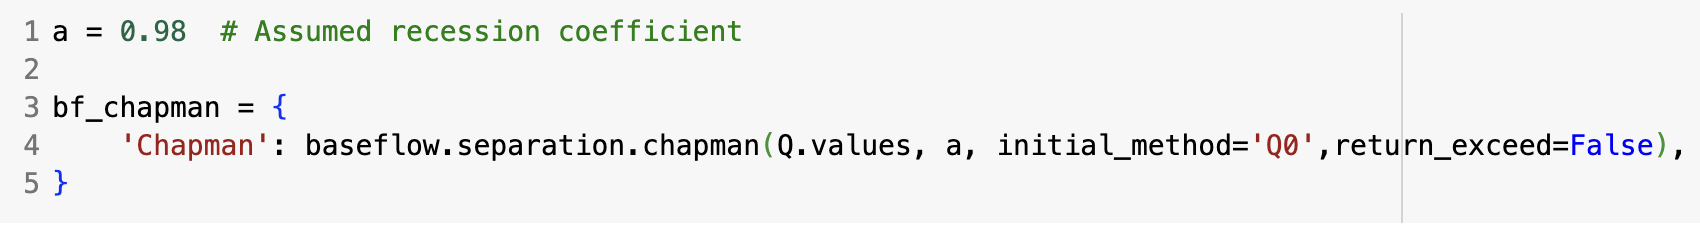
\includegraphics[width=0.8\textwidth]{figures/fig2.png}
\caption{The example usage of the Chapman method.\label{fig:chapman_usage}}
\end{figure}

The separation results are as follows: the baseflow values are returned for the same dates as the corresponding streamflow data. The two series are illustrated in Figure~\ref{fig:chapman_results}.

\begin{figure}[H]
\centering
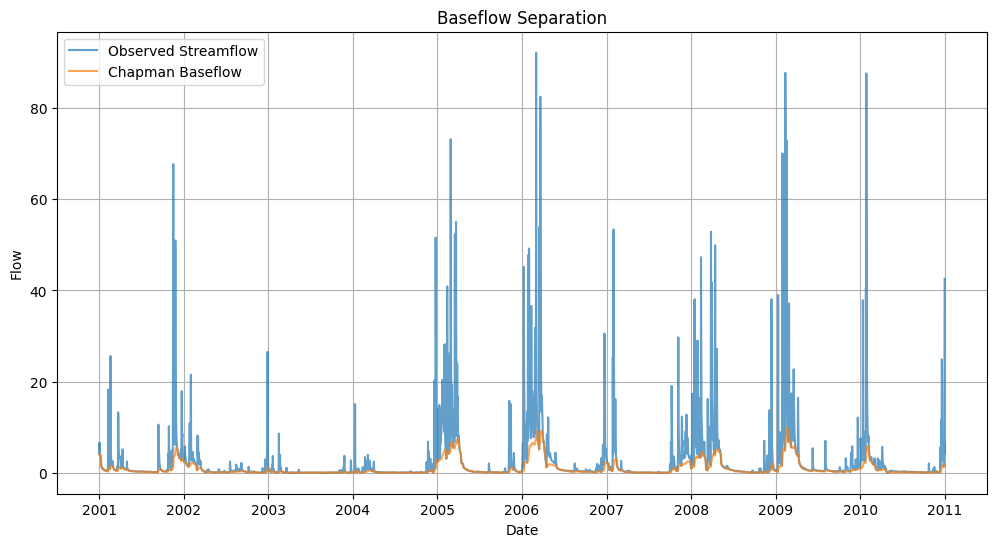
\includegraphics[width=0.8\textwidth]{figures/fig3.png}
\caption{Chapman baseflow separation results.\label{fig:chapman_results}}
\end{figure}

This standardized approach not only simplifies the use of individual methods but also facilitates comparative studies across multiple techniques, a crucial aspect in hydrological research where method selection can significantly impact results.

\subsection{Utility Functions}
\label{sec:utility_functions}

For the precise application, we add a \texttt{utils.py} file containing several utility functions that are essential for preprocessing and analyzing streamflow data within the baseflow package (Table~\ref{tab:utility}).

\begin{table}[H]
\caption{Functions in the Utility module.\label{tab:utility}}
\small
\begin{tabularx}{\textwidth}{lXXX}
\toprule
\textbf{Function} & \textbf{Description} & \textbf{Inputs} & \textbf{Outputs} \\
\midrule
clean\_streamflow & Preprocesses streamflow data by removing invalid entries and retaining years with sufficient data points. & series (pandas.Series): The streamflow time series to be cleaned. & tuple: Cleaned streamflow values and corresponding dates. \\
\addlinespace
exist\_ice & Identifies periods affected by ice conditions, providing a boolean mask for exclusion from analysis. & date (datetime.datetime): The date to check. ice\_period (tuple or numpy.ndarray): The ice period. & bool or numpy.ndarray: Boolean mask indicating ice presence. \\
\addlinespace
moving\_average & Smooths time series data by calculating the average over a specified window. & data (list): The data to be smoothed. window\_size (int): The size of the moving window. & list: The moving averages. \\
\addlinespace
multi\_arange & Generates a sequence of integers between specified start and stop values for each element in the input arrays. & starts (numpy.ndarray): Start values. stops (numpy.ndarray): Stop values. & numpy.ndarray: Sequence of integers. \\
\addlinespace
geo2imagexy & Converts geographic coordinates into image coordinates for spatial data integration. & x (float): The x-coordinate. y (float): The y-coordinate. & tuple: Column and row indices. \\
\addlinespace
format\_method & Standardizes the input method parameter into a consistent format for subsequent processing. & method (str or list): The input method parameter. & list: List of method names. \\
\addlinespace
kge & Calculates the Kling--Gupta Efficiency (KGE) and its components for evaluating hydrological model performance. & simulations (numpy.ndarray): Simulated data. evaluation (numpy.ndarray): Observed data. & float: KGE value and its components. \\
\bottomrule
\end{tabularx}
\end{table}

The \texttt{clean\_streamflow} function preprocesses streamflow time series data by removing invalid entries and retaining only the years with enough valid data points, ensuring the dataset's reliability and robustness for subsequent analysis. The \texttt{exist\_ice} function identifies periods within the dataset that are affected by ice conditions, providing a Boolean mask to facilitate the exclusion of these periods from analysis, which is crucial for maintaining the integrity of hydrological studies.

To smooth time series data and highlight underlying trends, the \texttt{moving\_average} function calculates the average over a specified window, making the data more interpretable and suitable for further analysis. The \texttt{multi\_arange} function enhances the efficiency of data handling by generating a sequence of integers between specified start and stop values for each element in the input arrays, which is particularly useful for creating index ranges for batch processing in numerical computations.

For integrating spatial data with grid-based or image-based datasets, the \texttt{geo2imagexy} function converts geographic coordinates into image coordinates, enabling the visualization and analysis of geographic information within a unified framework. The \texttt{format\_method} function standardizes the input method parameter into a consistent format, ensuring that the method list is prepared correctly for subsequent processing, which enhances the flexibility and usability of the package.

Finally, the \texttt{kge} function calculates the Kling--Gupta Efficiency (KGE) along with its components: correlation, variability ratio, and bias ratio. The KGE is a comprehensive metric for evaluating the performance of hydrological models, providing insights into the accuracy and reliability of simulated streamflow data compared to observed data.

%%%%%%%%%%%%%%%%%%%%%%%%%%%%%%%%%%%%%%%%%%
\section{Examples and Discussion}
\label{sec:examples}

\subsection{Development Methods}
\label{sec:development}

This section briefly introduces the essential packages required to set up the baseflow package. The accompanying Figure~\ref{fig:packages} illustrates all the necessary packages that constitute the baseflow package. These modules ensure that the package is both functional and reliable. We use commonly recognized abbreviations to keep it concise and accessible to a broader audience.

\begin{figure}[H]
\centering
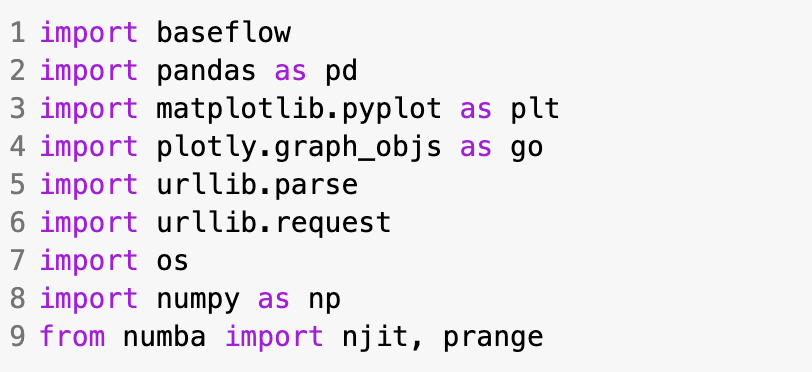
\includegraphics[width=0.6\textwidth]{figures/fig4.png}
\caption{Necessary packages to set up the baseflow package.\label{fig:packages}}
\end{figure}

\subsection{Data Preparation}
\label{sec:data_preparation}

Unlike some other online tools or local scripts that require users to manually open their local data files---a process that can be time-consuming and challenging with large datasets---we offer multiple methods for data preparation.

After installation, users can input their local data files in CSV format or any other format, as the reading functions in the code can be modified to accommodate different formats. Additionally, the package supports processing data for both single and multiple stations, allowing users to upload individual files or files containing data from multiple stations.

Second, we provide code in the Colab Notebook examples that enables users to retrieve daily streamflow data directly from the USGS website. By simply entering the station ID, start date, and end date, users can obtain clean streamflow data, free from any extraneous text, in a format that is ready for immediate use in subsequent calculation steps. This data is already structured to match our input format requirements.

\subsection{Pre-Processing}
\label{sec:preprocessing}

Once the original streamflow data has been input, it is crucial to perform pre-processing to ensure the data's quality and reliability before proceeding with further analysis. To facilitate this, we provide a function called \texttt{clean\_streamflow} in the \texttt{utils} module that handles the data preparation.

The \texttt{clean\_streamflow} function first removes any NaN values, which typically indicate missing observations or errors on those particular days. This step is essential to avoid inaccuracies in the subsequent analysis. Additionally, to ensure the robustness of the dataset, the function filters out any years with fewer than 120 recorded days (approximately one-third of a year). This threshold helps guarantee that the time series contains sufficient data points for meaningful analysis.

After cleaning the data, the function rearranges the streamflow values in chronological order, aligning them with their corresponding dates. This organized and cleaned dataset is then ready for use in further baseflow separation and other hydrological analyses.

\subsection{Example Usage}
\label{sec:example_usage}

On our documentation website, users can find links to Google Colab Notebooks that provide practical examples of how to use the package. We offer Notebooks for both single station and multiple station analyses, each accompanied by detailed descriptions of every step. These examples are designed to be interactive, allowing users to adjust parameters specific to their datasets and obtain results directly online.

As mentioned earlier, there are two primary methods for preparing the input streamflow data: using local files or retrieving data directly from the USGS website. For users who choose to upload their local datasets, we have made the process even more accessible by including a sample CSV file within the package. This example file allows users to quickly experience the usage procedure and explore the features of the package without needing to prepare their own data initially.

In the single station example, it focuses on a single station, demonstrating two methods to obtain data: using a local file and retrieving data from the USGS API.

For the local file method, the file can be added to the sidebar in the Colab interactive graphical tool in this example (Figure~\ref{fig:upload}). This file should be in CSV format, containing two columns: date and streamflow.

\begin{figure}[H]
\centering
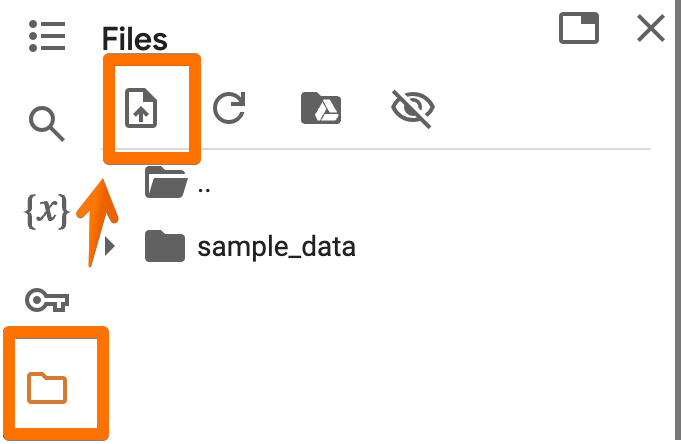
\includegraphics[width=0.5\textwidth]{figures/fig5.png}
\caption{Upload your own data.\label{fig:upload}}
\end{figure}

The package's \texttt{example.csv} serves as an illustration. The \texttt{pd.read\_csv} function from the Pandas package is employed to examine the file's content. The example data content is presented as follows:

\begin{figure}[H]
\centering
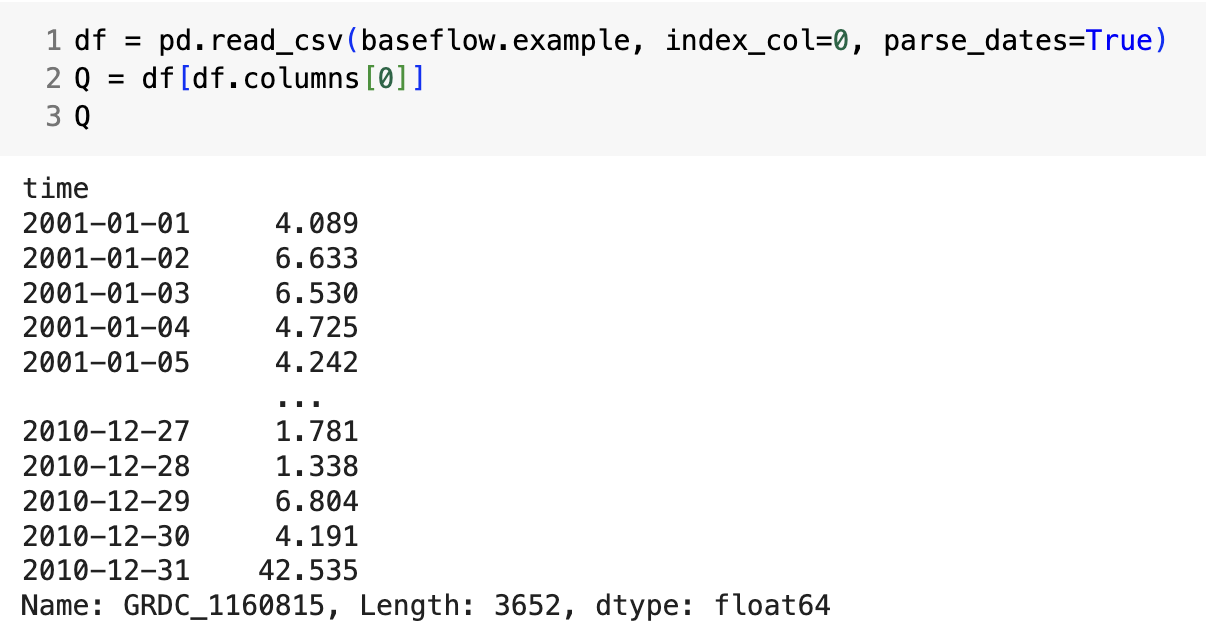
\includegraphics[width=0.6\textwidth]{figures/fig6.png}
\caption{The content of the example data.\label{fig:example_data}}
\end{figure}

For the USGS API, station ID 01636500 at Shenandoah River in Millville, WV is used as an illustrative example. We just need to type the information of the site in the following code block (Figure~\ref{fig:usgs_input}). It will return the link of this site data from USGS, and format it to the DataFrame with date and streamflow in the same format as the local file method.

\begin{figure}[H]
\centering
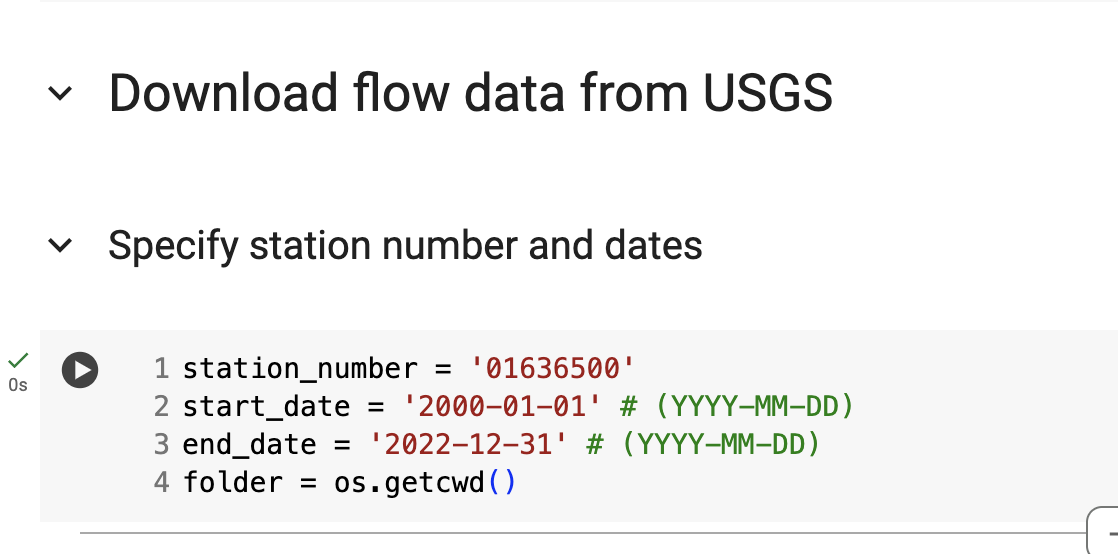
\includegraphics[width=0.8\textwidth]{figures/fig7.png}
\caption{Type the required input.\label{fig:usgs_input}}
\end{figure}

Figure~\ref{fig:timeseries} illustrates the time series of daily streamflow data from this station within the selected time range, post data cleaning.

\begin{figure}[H]
\centering
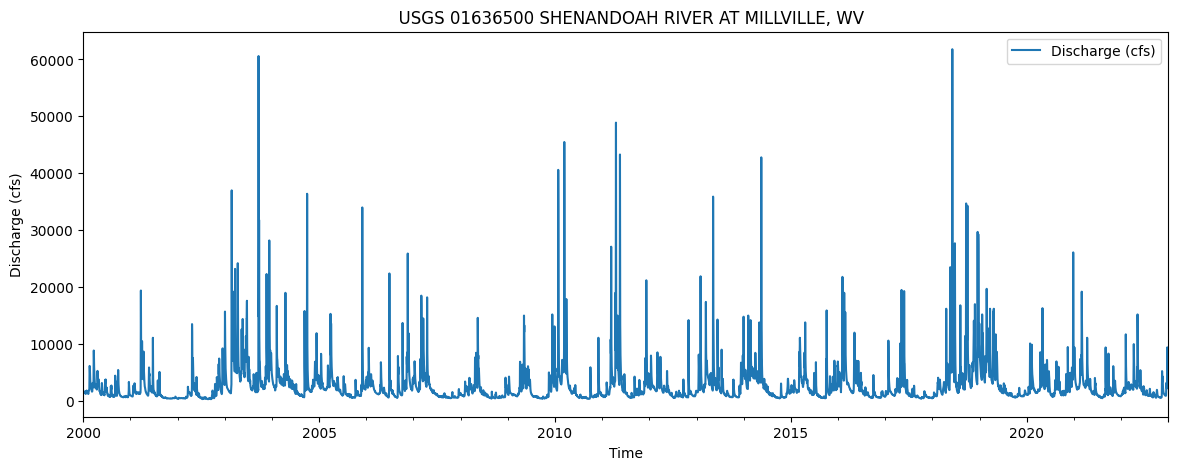
\includegraphics[width=0.8\textwidth]{figures/fig8.png}
\caption{The time series of the example USGS station.\label{fig:timeseries}}
\end{figure}

While this example primarily utilizes a single \texttt{single} function, it effectively demonstrates the collaboration of functions within the package. After loading the necessary packages, plotting functions are imported for further analysis. The initial step involves using the \texttt{clean\_up} function to ensure data quality. Subsequently, the original streamflow data is visualized to discern its features, such as curves and trends.

Post-preprocessing, the \texttt{single} function is employed to compute results using selected methods. This function requires three parameters: \texttt{series} for streamflow data, \texttt{method} for the chosen separation method, and \texttt{return\_kge} to return KGE values (optional).

During calculation, the \texttt{lyne\_hollick} method initially computes the baseflow value, if required by the selected method, and calculates coefficient values for enhanced accuracy. The subsequent steps involve invoking corresponding methods from the \texttt{baseflow.separation} module, returning results alongside optional KGE values. This streamlined approach enables the computation of one or multiple methods concurrently, or even all methods included in the package, using a single line of code. The code requires streamflow as a \texttt{pandas.Series} and the desired method as a float. KGE is optional. The results are presented as follows (Figure~\ref{fig:results}).

\begin{figure}[H]
\centering
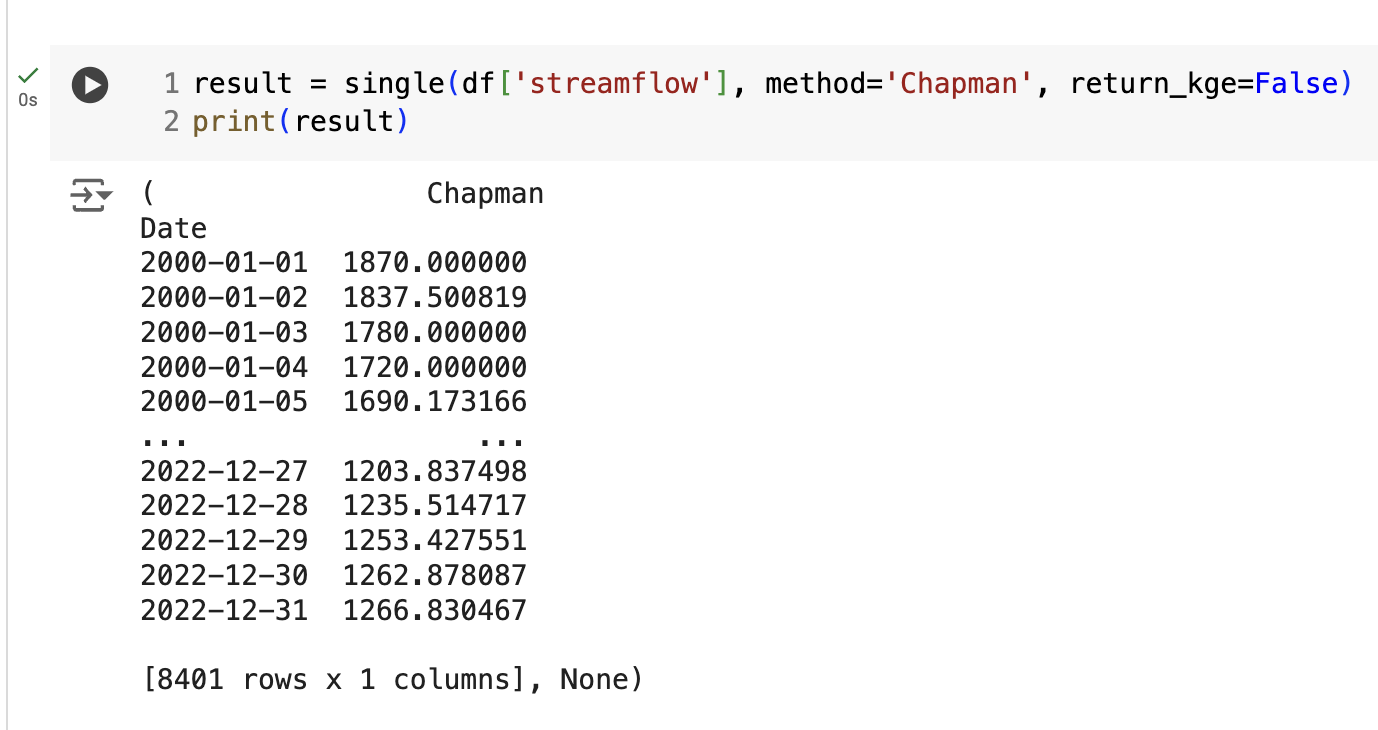
\includegraphics[width=0.45\textwidth]{figures/fig9a.png}
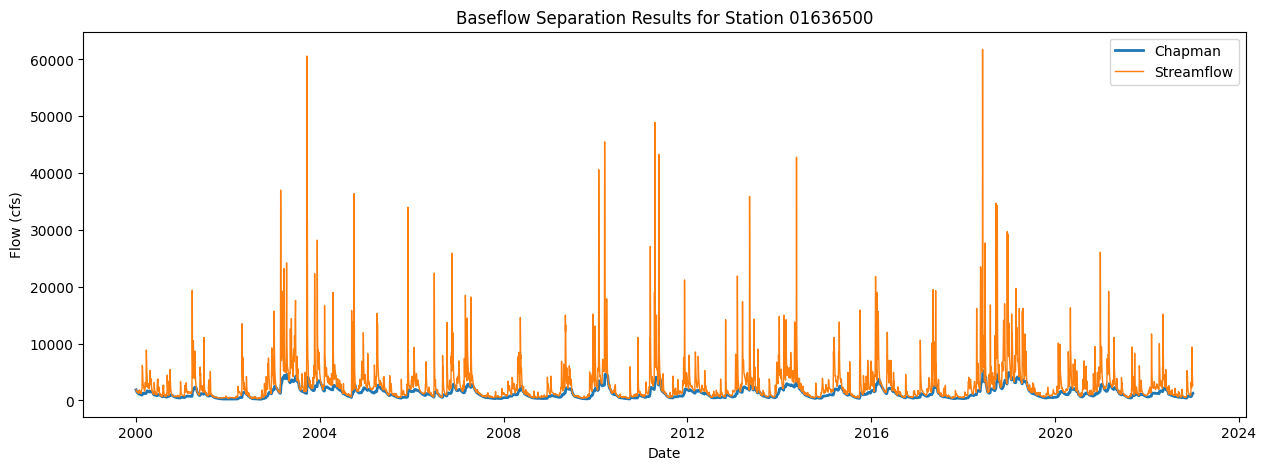
\includegraphics[width=0.45\textwidth]{figures/fig9b.png}
\caption{The separation outcome on a single station.\label{fig:results}}
\end{figure}

In addition, we provide a Colab notebook and have created a function to perform calculations for multiple stations, which serves as an example for situations where users need to apply these functions simultaneously to several stations. This function includes the single-station functionality, with the added capability of handling multiple stations by incorporating station-specific information, such as the station ID.

%%%%%%%%%%%%%%%%%%%%%%%%%%%%%%%%%%%%%%%%%%
\section{Conclusions}
\label{sec:conclusions}

This open-source baseflow package offers a straightforward and accessible solution for separating baseflow from streamflow data. Unlike outdated R code commonly found online, this package leverages the flexibility of the widely-used Python programming language, making it adaptable to various applications.

Users have multiple options for inputting data. While the traditional method involves uploading local CSV files, our package also allows users to directly access USGS stream station data through our API functions. Importantly, we provide not only the source code on GitHub and comprehensive documentation on ReadTheDocs, but also Google Colab Notebooks as examples of how to use the package. This setup ensures maximum convenience, enabling users to modify parameters and process their data online to obtain results efficiently.

We provide detailed examples in Google Colab Notebooks to demonstrate various application scenarios. These examples show how to apply the package to either a single station or multiple stations, using local data files or by directly downloading USGS data through our API functions. This enables users to calculate results using different methods on single or multiple datasets simultaneously.

Google Colab serves as an online platform where code can be executed with ease. Users can run code cells that are accompanied by descriptions provided before each code block. This setup allows users to modify parameters and obtain results directly within the online tool, without needing to install the package or run it in an IDE on their local machines.

We aim for this package to serve as a user-friendly tool for hydrology engineers and researchers. Additionally, we hope it will foster a community for potential collaboration and further development.

%%%%%%%%%%%%%%%%%%%%%%%%%%%%%%%%%%%%%%%%%%
\section{Discussion}
\label{sec:discussion}

The package structure is designed to be intuitive, with separation methods grouped under the \texttt{separation} module and utility functions under the \texttt{utils} module. Additionally, the \texttt{Estimate} module is dedicated to calculating related helper functions.

We provide detailed documentation of the baseflow package using markdown documents on GitHub which are then rendered using the readthedocs.io platform.

Source code is available at the project home page:
\url{https://github.com/BYU-Hydroinformatics/baseflow/}

Detailed documentation and references are available at:
\url{https://baseflow.readthedocs.io/en/latest/}

%%%%%%%%%%%%%%%%%%%%%%%%%%%%%%%%%%%%%%%%%%
\vspace{6pt}

%%%%%%%%%%%%%%%%%%%%%%%%%%%%%%%%%%%%%%%%%%
%% optional
%\supplementary{The following supporting information can be downloaded at: \linksupplementary{s1}}

%%%%%%%%%%%%%%%%%%%%%%%%%%%%%%%%%%%%%%%%%%
\authorcontributions{Conceptualization, N.J. and T.P.C.; methodology, X.L. and A.A.; software, X.L., A.A., J.H., A.K. and B.B.; validation, X.L. and A.A.; writing---original draft preparation, X.L.; writing---review and editing, N.J., G.W., D.R. and T.P.C.; supervision, N.J. and T.P.C. All authors have read and agreed to the published version of the manuscript.}

\funding{This research received no external funding.}

%\informedconsent{}

\dataavailability{The baseflow Python package is publicly available at \url{https://github.com/BYU-Hydroinformatics/baseflow/}. Documentation is available at \url{https://baseflow.readthedocs.io/en/latest/}.}

\conflictsofinterest{The authors declare no conflicts of interest.}

%%%%%%%%%%%%%%%%%%%%%%%%%%%%%%%%%%%%%%%%%%
\begin{adjustwidth}{-\extralength}{0cm}

\reftitle{References}

\begin{thebibliography}{99}

\bibitem{ref1}
Chapman, T.; Maxwell, A. Baseflow Separation---Comparison of Numerical Methods with Tracer Experiments. \textit{Hydrol. Water Resour. Symp.} \textbf{1996}.

\bibitem{ref2}
Chen, H.; Teegavarapu, R.S.V. Comparative Analysis of Four Baseflow Separation Methods in the South Atlantic-Gulf Region of the U.S. \textit{Water} \textbf{2020}, \textit{12}, 120. \url{https://doi.org/10.3390/w12010120}

\bibitem{ref3}
Lyne, V. Stochastic Time-Variable Rainfall-Runoff Modelling. \textit{Inst. Eng. Aust. Natl. Conf. Publ.} \textbf{1979}, \textit{79}, 89--93.

\bibitem{ref4}
Chapman, T.G. Comment on ``Evaluation of Automated Techniques for Base Flow and Recession Analyses'' by R.~J. Nathan and T.~A. McMahon. \textit{Water Resour. Res.} \textbf{1991}, \textit{27}, 1783--1784. \url{https://doi.org/10.1029/91WR01007}

\bibitem{ref5}
Eckhardt, K. How to Construct Recursive Digital Filters for Baseflow Separation. \textit{Hydrol. Process.} \textbf{2005}, \textit{19}, 507--515. \url{https://doi.org/10.1002/hyp.5675}

\bibitem{ref6}
Sloto, R.; Crouse, M. HYSEP---A Computer Program for Streamflow Hydrograph Separation and Analysis. \textit{US Geol. Surv. Water Resour. Invest. Rep.} \textbf{1996}, 96--4040.

\bibitem{ref7}
Piggott, A.R.; Moin, S.; Southam, C. A Revised Approach to the UKIH Method for the Calculation of Baseflow. \textit{Hydrol. Sci. J.} \textbf{2005}, \textit{50}, 911--920. \url{https://doi.org/10.1623/hysj.2005.50.5.911}

\bibitem{ref8}
Shao, G.; Zhang, D.; Guan, Y.; Sadat, M.A.; Huang, F. Application of Different Separation Methods to Investigate the Baseflow Characteristics of a Semi-Arid Sandy Area, Northwestern China. \textit{Water} \textbf{2020}, \textit{12}, 434. \url{https://doi.org/10.3390/w12020434}

\bibitem{ref9}
Ramli, I.; Murthada, S.; Nasution, Z.; Achmad, A. Hydrograph Separation Method and Baseflow Separation Using Chapman Method---A Case Study in Peusangan Watershed. \textit{IOP Conf. Ser. Earth Environ. Sci.} \textbf{2019}, \textit{314}, 012026. \url{https://doi.org/10.1088/1755-1315/314/1/012026}

\bibitem{ref10}
Abdi, D.M. Performance Analysis of Baseflow Separation Methods: The Case of Rift Valley Lakes Basin, Ethiopia. \textit{Indones. J. Earth Sci.} \textbf{2022}, \textit{2}, 145--156. \url{https://doi.org/10.52562/injoes.v2i2.451}

\bibitem{ref11}
Boughton, W.C. A Hydrograph-Based Model for Estimating the Water Yield of Ungauged Catchments. \textit{Hydrol. Water Resour. Symp. Newcastle, IEAust} \textbf{1993}.

\bibitem{ref12}
Tularam, G.A.; Ilahee, M. Exponential Smoothing Method of Base Flow Separation and Its Impact on Continuous Loss Estimates. \textit{Am. J. Environ. Sci.} \textbf{2008}, \textit{4}, 136--144. \url{https://doi.org/10.3844/ajessp.2008.136.144}

\bibitem{ref13}
Sarailidis, G.; Vasiliades, L.; Loukas, A. Analysis of Streamflow Droughts Using Fixed and Variable Thresholds. \textit{Hydrol. Process.} \textbf{2019}, \textit{33}, 414--431. \url{https://doi.org/10.1002/hyp.13336}

\bibitem{ref14}
Furey, P.R.; Gupta, V.K. A Physically Based Filter for Separating Base Flow from Streamflow Time Series. \textit{Water Resour. Res.} \textbf{2001}, \textit{37}, 2709--2722. \url{https://doi.org/10.1029/2001WR000243}

\bibitem{ref15}
Ladson, T. A Standard Approach to Baseflow Separation Using the Lyne and Hollick Filter. \textit{Aust. J. Water Resour.} \textbf{2013}, \textit{17}, 25--34. \url{https://doi.org/10.7158/W12-028.2013.17.1}

\bibitem{ref16}
Li, L.; Maier, H.R.; Lambert, M.F.; Simmons, C.T.; Partington, D. Framework for Assessing and Improving the Performance of Recursive Digital Filters for Baseflow Estimation with Application to the Lyne and Hollick Filter. \textit{Environ. Model. Softw.} \textbf{2013}, \textit{41}, 163--175. \url{https://doi.org/10.1016/j.envsoft.2012.11.009}

\bibitem{ref17}
Qiao, X.; Nelson, E.J.; Ames, D.P.; Li, Z.; David, C.H.; Williams, G.P.; Roberts, W.; Lozano, J.L.S.; Edwards, C.; Souffront, M. A Systems Approach to Routing Global Gridded Runoff through Local High-Resolution Stream Networks for Flood Early Warning Systems. \textit{Environ. Model. Softw.} \textbf{2019}, \textit{120}, 104501.

\bibitem{ref18}
Anderson, D.L.; Ames, D.P.; Yang, P. Quantitative Methods for Comparing Different Polyline Stream Network Models. \textit{J. Geogr. Inf. Syst.} \textbf{2014}. \url{https://doi.org/10.4236/jgis.2014.62010}

\bibitem{ref19}
Ames, D.P.; Li, Z.; Qiao, X.; Tarboton, D.G.; Idaszak, R.; Horsburgh, J.S.; Merwade, V.; Miles, B.; Swain, N.R.; Lineberger, R.; et~al. Web-Based Data Visualization and Analysis Using HydroShare and the Open Source Tethys Platform. \textit{AGU Fall Meet. Abstr.} \textbf{2015}, \textit{43}, H43A-1473.

\bibitem{ref20}
Cheng, L.; Zhang, L.; Brutsaert, W. Automated Selection of Pure Base Flows from Regular Daily Streamflow Data: Objective Algorithm. \textit{J. Hydrol. Eng.} \textbf{2016}, \textit{21}, 06016008. \url{https://doi.org/10.1061/(ASCE)HE.1943-5584.0001427}

\bibitem{ref21}
Xie, J.; Liu, X.; Wang, K.; Yang, T.; Liang, K.; Liu, C. Evaluation of Typical Methods for Baseflow Separation in the Contiguous United States. \textit{J. Hydrol.} \textbf{2020}, \textit{583}, 124628. \url{https://doi.org/10.1016/j.jhydrol.2020.124628}

\bibitem{ref22}
Ladson, T. A Standard Approach to Baseflow Separation Using the Lyne and Hollick Filter. \textit{Aust. J. Water Resour.} \textbf{2013}, \textit{17}, 25--34.

\end{thebibliography}

\end{adjustwidth}

\end{document}
